%% Thesis template
%% PMC, University of Minho
%% if required, comment unused packages
\documentclass[12pt,english]{book}
% \usepackage[portuguese]{babel}
% \usepackage[utf8]{inputenc} 
\usepackage{times}
\usepackage[T1]{fontenc}
\usepackage[latin1]{inputenc}
\usepackage{a4wide}
\usepackage{fancyhdr}
\pagestyle{fancy}
\usepackage{subfigure}
\usepackage{float}
\usepackage{graphicx}
\usepackage{setspace}
\usepackage{cite}\onehalfspacing

\makeatletter

%%%%%%%%%%%%%%%%%%%%%%%%%%%%%% LyX specific LaTeX commands.
%% Bold symbol macro for standard LaTeX users
\newcommand{\boldsymbol}[1]{\mbox{\boldmath $#1$}}

\floatstyle{ruled}
\newfloat{algorithm}{tbp}{loa}
\floatname{algorithm}{Algorithm}

%%%%%%%%%%%%%%%%%%%%%%%%%%%%%% Textclass specific LaTeX commands.
 \usepackage{verbatim}
 \newenvironment{lyxlist}[1]
   {\begin{list}{}
     {\settowidth{\labelwidth}{#1}
      \setlength{\leftmargin}{\labelwidth}
      \addtolength{\leftmargin}{\labelsep}
      \renewcommand{\makelabel}[1]{##1\hfil}}}
   {\end{list}}

%%%%%%%%%%%%%%%%%%%%%%%%%%%%%% User specified LaTeX commands.
\usepackage{color}
\usepackage{colortbl}
\usepackage{url}
\input{epsf}
\newcommand{\single}{\renewcommand\baselinestretch{1.0}}
\newcommand{\onehalf}{\renewcommand\baselinestretch{1.5}}
\newcommand{\double}{\renewcommand\baselinestretch{2.0}}
\fancyhead{}
\fancyhead[LE]{\slshape \leftmark}
\fancyhead[RO]{\slshape \rightmark}
\cfoot{\thepage}
\setlength{\parskip}{2mm}

\usepackage{babel}
\makeatother
\begin{document}
\begin{minipage}[c]{1.0\columnwidth}%
\begin{doublespace}
\vspace{2cm}
\begin{center}{\huge A new Framework to enable rapid innovation in Cloud Datacenter through a SDN approach.}\end{center}{\huge \par}
\end{doublespace}

\vspace{2cm}
\begin{center}{\large Jos\'{e} Teixeira}\end{center}{\large \par}
\vspace{2cm}

\begin{quote}
\begin{center}A thesis submitted to the University of Minho in the
subject of Informatics, for the degree of
% or Doctor of Philosophy 
Master of Science, under scientific supervision of Prof. Stefano Giordano and Prof. Alexandre Santos\end{center}\vspace{3cm}

\end{quote}
\begin{singlespace}
\begin{center}University of Minho\end{center}

\begin{center}School of Engineering\end{center}

\begin{center}Department of Informatics\end{center}
\end{singlespace}

\begin{center}{\large September, 2013}\end{center}\end{minipage}%
\thispagestyle{empty}

\pagenumbering{roman}


\newpage


\chapter*{Acknowledgments}

\addcontentsline{toc}{chapter}{Acknowledgments}

\noindent I would like...

\medskip{}
\noindent I also...

\chapter*{Abstract}

\addcontentsline{toc}{chapter}{Abstract}

\begin{singlespace}
In the last years, the widespread of Cloud computing as the main paradigm to deliver a large plethora of virtualized services significantly increased the complexity of Datacenters management and raised new performance issues for the intra-Datacenter network.
Providing heterogeneous services and satisfying users' experience is really challenging for Cloud service providers, since system (IT resources) and network administration functions are definitely separated.

As the Software Defined Networking (SDN) approach seems to be a promising way to address innovation in Datacenters, the thesis presents a new framework that allows to develop and test new OpenFlow--based controllers for Cloud Datacenters.
More specifically, the framework enhances both Mininet (a well--known SDN emulator) and POX (a Openflow controller written in python), with all the extensions necessary to experiment novel control and management strategies of IT and network resources.

... talk about obtained results and conclusions(not finished yet, complete when you finish everything)

\end{singlespace}

\paragraph{Keywords:}
Datacenter, Cloud, SDN, OpenFlow.

\newpage

\cleardoublepage

\addcontentsline{toc}{chapter}{Contents}\tableofcontents{}

\cleardoublepage

\chapter*{List of Acronyms}

\addcontentsline{toc}{chapter}{List of Acronyms}

\markboth{LIST OF ACRONYMS}{LIST OF ACRONYMS}

\begin{lyxlist}{00.00.0000}
\begin{singlespace}
\item [DC]Datacenter
\item [SDN]Software Defined Networking
\item [OF]Openflow
\item [VM]Virtual Machine
\item [IP]Internet Protocol 
\item Add as needed...
\end{singlespace}
\end{lyxlist}

\cleardoublepage

\addcontentsline{toc}{chapter}{List of Figures}\listoffigures

\cleardoublepage

\addcontentsline{toc}{chapter}{List of Tables}\listoftables

\cleardoublepage

\setcounter{page}{0}

\pagenumbering{arabic}


\chapter{Introduction\label{cha:introduction}}

\section{Introduction}

A Cloud DC consists of virtualized resources that are dynamically allocated, in a seamless and automatic way, to a plethora of heterogeneous applications.
In Cloud DCs, services are no more tightly bounded to physical servers, as occurred in traditional DCs, but are provided by Virtual Machines that can migrate from a physical server to another increasing both scalability and reliability.
Software virtualization technologies allow a better usage of DC resources; DC management, however, becomes much more difficult, due to the strict separation between systems (\textit{i.e.}, server, VMs and virtual switches) and network (\textit{i.e.}, physical switches) administration.

Moreover, new issues arise, such as isolation and connectivity of VMs.
Services performance may suffer from the fragmentation of resources as well as the rigidity and the constraints imposed by the intra-DC network architecture (usually a multilayer 2-tier or 3-tier fat-tree composed of Edge, Aggregation and Core switches\cite{dc_arch}).
Therefore, Cloud service providers (\textit{e.g.},\cite{amazon}) ask for a next generation of intra-DC networks meeting the following features: 1) efficiency, \textit{i.e.}, high server utilization; 2) agility, \textit{i.e.}, fast network response to server/VMs provisioning; 3) scalability, \textit{i.e.}, consolidation and migration of VMs based on applications' requirements; 4) simplicity, \textit{i.e.}, performing all those tasks easily\cite{baldonado}.

In this scenario, a recent approach to programmable networks (\textit{i.e.}, Software-Defined Networking) seems to be a promising way to satisfy DC network requirements\cite{ibmnec}. 
Unlike the classic approach where network devices forward traffic according to the adjacent devices, SDN is a new network paradigm that decouples routing decisions (control plane) from the traffic forwarding (data plane). This routing decisions are made by a programmable centralized intelligence called controller that helps make this architecture more dynamic, automated and manageable.

Following the SDN--based architecture the most deployed SDN protocol is OpenFlow\cite{openflow}\cite{onf}, as it is the open standard protocol to communicate and control OF-compliant network devices.
[continue later with the same logic as the sentence below]
 that allows to set into OF--compliant switches forwarding rules established by a centralized intelligence called controller.

Since SDN allows to re-define and re-configure network functionalities (possibly up to the physical layer), the basic idea is to introduce an SDN-cloud-DC controller that enables a more efficient, agile, scalable and simple use of both VMs and network resources.
Nevertheless, before deploying the novel architectural solutions, huge test campaigns must be performed in experimental environments reproducing a real DC.

To this aim, a novel framework is introduced that allows to develop and assess novel SDN-Cloud-DC controllers, and to compare the performance of control and management strategies jointly considering both IT and network resources\cite{im2013}.

% \pagebreak
\section{Motivation and objectives\label{sec:motobj}}

Being the 
\begin{itemize}
	\item Understanding the basic features of SDN paradigm
	\item Studying the problematics in cloud DC VM allocations
	\item Apply the SDN paradigm to better exploit the DC resources
	\item Develop a framework for Cloud Datacenter emulation and new VM allocation policies
	\item ...
\end{itemize}

\section{Dissertation layout}

In the present Chapter \ref{cha:introduction} - ...

\chapter{State of art \label{cha:stateofart} }

Usually background and related work ...

\section{Available solutions}

Write something generic

\subsection{CloudSim}

Calheiros et al.[6] proposed a Java-based platform, called Cloudsim, that allows to estimate cloud servers performance using a workflow model to simulate applications behaviour. 

\subsection{NetFPGA Emulation}

Ellithorpe et al.[7] proposed, an FPGA emulation platform that allows to emulate up-to 256 network nodes on a single chip. However, the cost of a single board is approximately 2, 000 dollars making this solution less attractive than one based on open--source software.

\subsection{Meridian}

Following the new shiny SDN paradigm, Banikazemi et al.[4] proposed Meridian, an SDN--based controller
framework for cloud services in real environments: such a platform allows to create and manage different kind
of logical network topologies, but it works on top of a cloud Iaas platform (i.e., Openstack[18], IBM Smart
Cloud Provisioning[9]) while our solution is a flexible, standalone software that could even run in a virtualized environment.

\subsection{Networkcloudsim, Greencloud and icancloud}

Other well--known open--source cloud simulators are[13][11] and[19], but in none of them (even in Cloudsim) SDN features are available.

\newpage
\section{Openflow Controllers}

\newpage
\section{Virtual Machine Allocation Policies}

\newpage
\section{Virtual Machine Migration Policies}

\newpage
\section{QoS in SDN}
\newpage

% Uncomment to include file.pdf
%\begin{figure}%[H]
%\begin{center}\includegraphics[scale=0.8]{file}\end{center}
%\caption{Legend \label{fig:LABEL}}
%\end{figure}


\chapter{The Framework \label{cha:framework} }

Provide the user with a full package for the development and test of DC SDN Controller was one of the main purposes of the framework.
Aiming for such goal, but without discarding the deployment in a real DC, a single software environment was designed and developed.
Because the requirements change according to the controller being in the development or the deployment phase, so does the environment in order to best suit each of them.

\section{Requirements}

Explain the different requirements in a development \& test versus deployment phase.

This environment can be seen as two main components: the DC oriented controller and the DC Topology.

The first one, a full featured python controller for OF switches called POX was used as groundwork. It has ready-to-use modules that are helpful when it comes to making a controller, as they provide some abstraction.
However, POX API is too low level for a user that aims to implement a new DC controller, which prevents the rapid development of the logic thought by the user.
To fill this gap, the controller available in the framework includes all the abstraction levels needed for quickly building a DC oriented controller while still being fully dynamic.

As for the second component, since performing tests and debug in a real topology can be challenging operations

the starting point was Mininet, a network emulator for SDN systems, which provides an API to reproduce any kind of topology without the need of hardware resources.
Therefore, Mininet enables the assessment of the operation of an OF controller before its deployment in a real environment.
Despite its flexibility, Mininet lacks of a complete set of tools that easily allow to emulate the behaviour of a cloud DC, thus raising the following questions:
 
\begin{itemize}
\item How to easily generate and configure typical DC topologies?
\item How to simulate VMs allocation requests?
\item How to emulate the inter and in/out DC traffic?
\end{itemize}


\section{Framework architecture}

\begin{figure}[htbp]
        \centering
        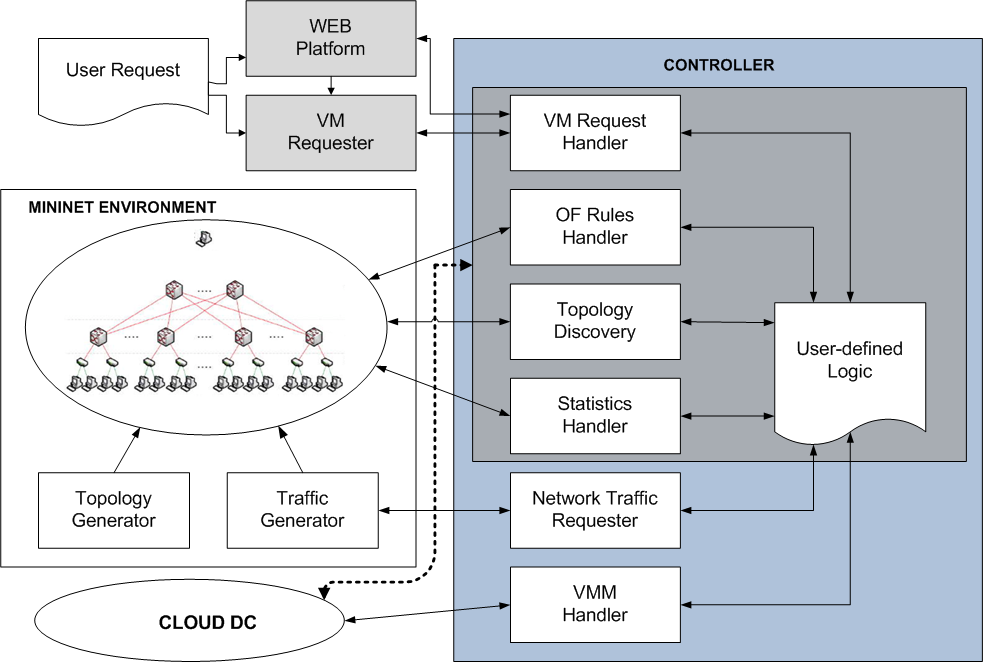
\includegraphics[width=0.7\textwidth]{figures/emulator_new.png}
        \caption{The framework}
        \label{fig:framework}
\end{figure}

\section{Framework modules: Mininet Environment}

\subsection{Topology Generator}

\subsection{Traffic Generator}

Describe each module, it's functionalities, limitations, how it can be used/improved (improved if the user wants to add new features)

\begin{itemize}
	\item Talk generally about the traffic generator
	\item Talk about the one's we tried (pros and cons)
\end{itemize}

\newpage


\section{Framework modules: Controller}

Describe each module, it's functionalities, limitations, how it can be used/improved (improved if the user wants to add new features)

\subsection{Topology Discovery}

\subsection{OF Rules Handler}

\subsection{Statistics Handler}

\subsection{VM Request Handler}

\subsection{VMM - Virtual Machines Manager}

\subsection{Network Traffic Requester}

\subsection{POX Modules}

\subsection{User Defined Logic}

\newpage


\section{Framework modules: Web Platform}

Describe each module, it's functionalities, limitations, how it can be used/improved (improved if the user wants to add new features)

\newpage


\section{Framework modules: VM Requester}

Describe each module, it's functionalities, limitations, how it can be used/improved (improved if the user wants to add new features)

\newpage


\section{Using the framework}

\subsection{Emulator}

Describe how to use the framework (emulation part) and how to access the API..

\subsection{Real Environment}

Describe what changes in the real environment (the modules that are disabled and the ones that need to be enabled)

\chapter{Framework extensions \label{cha:} }

\section{Enabling QoS}
\subsection{QoS in the framework}
\newpage

\section{Enabling Virtual Machine migration}
\subsection{Virtual Machine migration in the framework}
\subsection{Usecase}

\chapter{Validation and tests \label{cha:valtes} }

Usually test and validation of the proposed solution ...

\section{Framework Validation}

\begin{itemize}
	\item Show how Bf goes against WF with server driven algorithm (show server occupation)
	\item Show how Bf goes against WF with network driven algorithm (show network occupation) (although the behaviour is similar is allow to say that net algorithm may use switch statistics)
\end{itemize}
\newpage


\section{Performance Evaluation}

Get the tests from the submitted paper.
\newpage

\section{Real environment tests}
\begin{itemize}
	\item Talk about the environment which was setup
	\begin{itemize}
		\item Chosen hypervisor
		\item Talk about Xen api and the alternative solution (ssh each server and run a script to clone the vm)
		\item OpenVswitches VS NetFPGA problems
		\item 
	\end{itemize}
\end{itemize}
\newpage

\chapter{Conclusions\label{cha:conclusions}}

This chapter provides ...

\section{Main contributions}

\section{Future work}

\appendix

\chapter{Name of the Appendix}

\cleardoublepage

\markright{\slshape Appendix}

\cleardoublepage
\bibliographystyle{unsrt}
\addcontentsline{toc}{chapter}{\bibname}

%% Add file.bib
\bibliography{sigproc}
\nocite{*}



\end{document}

%Layout do Vasco
% 0- Resumo/abstract
% 1- Conceitos Introdutórios
% WebRTC (APIs W3C)x, ICEx/STUNx/TURNx, RTP/DTLSx, Codecs, Protocolos DataChannel (UDP - SCTPx - DTLSx), Sinalização (draft JSEP, SIP sobre WebSockets, Jingle sobre WebSockets), WebSockets
% 2- Estado da Arte
% soluções existentes:
% Libs javascript incl as Libs do Muaz
% Sinalização: node.js, vertx
% Gateways para SIP
% 3- Requisitos e Casos de Uso
% 4- Experimentação e Seleção de Soluções Existentes
% Node.js vs Vertx
% Libs do Muaz vs ?
% 5- Arquitectura e Desenho
% Especificação das APIs Javascript e do Servidor (manual para programador)
% 6- Validação e Testes
% Aplicação 
% 7- Conclusões